% vim: set spell spelllang=en tw=100 et sw=4 sts=4 foldmethod=marker foldmarker={{{,}}} :

\documentclass{beamer}

\usepackage{tikz}
\usepackage{xcolor}
\usepackage{complexity}
\usepackage{hyperref}
\usepackage{microtype}
\usepackage{amsmath}                   % \operatorname
\usepackage{amsfonts}                  % \mathcal
\usepackage{amssymb}                   % \nexists
\usepackage{gnuplot-lua-tikz}          % graphs
\usepackage[vlined]{algorithm2e} % algorithms
\usepackage{centernot}
\usepackage{graphicx}

\usetikzlibrary{shapes, arrows, shadows, calc, positioning, fit}
\usetikzlibrary{decorations.pathreplacing, decorations.pathmorphing, shapes.misc}
\usetikzlibrary{tikzmark}

\definecolor{uofguniversityblue}{rgb}{0, 0.219608, 0.396078}

\definecolor{uofgheather}{rgb}{0.356863, 0.32549, 0.490196}
\definecolor{uofgaquamarine}{rgb}{0.603922, 0.72549, 0.678431}
\definecolor{uofgslate}{rgb}{0.309804, 0.34902, 0.380392}
\definecolor{uofgrose}{rgb}{0.823529, 0.470588, 0.709804}
\definecolor{uofgmocha}{rgb}{0.709804, 0.564706, 0.47451}
\definecolor{uofgsandstone}{rgb}{0.321569, 0.278431, 0.231373}
\definecolor{uofgforest}{rgb}{0, 0.2, 0.129412}
\definecolor{uofglawn}{rgb}{0.517647, 0.741176, 0}
\definecolor{uofgcobalt}{rgb}{0, 0.615686, 0.92549}
\definecolor{uofgturquoise}{rgb}{0, 0.709804, 0.819608}
\definecolor{uofgsunshine}{rgb}{1.0, 0.862745, 0.211765}
\definecolor{uofgpumpkin}{rgb}{1.0, 0.72549, 0.282353}
\definecolor{uofgthistle}{rgb}{0.584314, 0.070588, 0.447059}
\definecolor{uofgrust}{rgb}{0.603922, 0.227451, 0.023529}
\definecolor{uofgburgundy}{rgb}{0.490196, 0.133333, 0.223529}
\definecolor{uofgpillarbox}{rgb}{0.701961, 0.047059, 0}
\definecolor{uofglavendar}{rgb}{0.356863, 0.301961, 0.580392}

\tikzset{vertex/.style={draw, circle, inner sep=0pt, minimum size=0.5cm, font=\small\bfseries}}
\tikzset{notvertex/.style={vertex, color=white, text=black}}
\tikzset{plainvertex/.style={vertex}}
\tikzset{vertexc1/.style={vertex, fill=uofgburgundy, text=white}}
\tikzset{vertexc2/.style={vertex, fill=uofgsandstone, text=white}}
\tikzset{vertexc3/.style={vertex, fill=uofgforest, text=white}}
\tikzset{vertexc4/.style={vertex, fill=uofgheather, text=white}}
\tikzset{edge/.style={color=black!50!white}}
\tikzset{bedge/.style={ultra thick}}

% {{{ theme things
\useoutertheme[footline=authortitle]{miniframes}
\useinnertheme{rectangles}

\setbeamerfont{block title}{size={}}
\setbeamerfont{title}{size=\large,series=\bfseries}
\setbeamerfont{section title}{size=\large,series=\mdseries}
\setbeamerfont{author}{size=\normalsize,series=\mdseries}
\setbeamercolor*{structure}{fg=uofguniversityblue}
\setbeamercolor*{palette primary}{use=structure,fg=black,bg=white}
\setbeamercolor*{palette secondary}{use=structure,fg=white,bg=uofgcobalt}
\setbeamercolor*{palette tertiary}{use=structure,fg=white,bg=uofguniversityblue}
\setbeamercolor*{palette quaternary}{fg=white,bg=black}

\setbeamercolor*{titlelike}{parent=palette primary}

\beamertemplatenavigationsymbolsempty

\setbeamertemplate{title page}
{
    \begin{tikzpicture}[remember picture, overlay]
        \node at (current page.north west) {
            \begin{tikzpicture}[remember picture, overlay]
                \fill [fill=uofguniversityblue, anchor=north west] (0, 0) rectangle (\paperwidth, -2.6cm);
            \end{tikzpicture}
        };

        \node (logo) [anchor=north east, shift={(-0.6cm,-0.6cm)}] at (current page.north east) {
            
\includegraphics[keepaspectratio=true,scale=0.7]{UoG_keyline.pdf}
        };

        \node [anchor=west, xshift=0.2cm] at (current page.west |- logo.west) {
            \begin{minipage}{0.65\paperwidth}\raggedright
                {\usebeamerfont{title}\usebeamercolor[white]{}\inserttitle}\\[0.1cm]
                {\usebeamerfont{author}\usebeamercolor[white]{}\insertauthor}
            \end{minipage}
        };
    \end{tikzpicture}
}

\setbeamertemplate{section page}
{
    \begin{centering}
        \begin{beamercolorbox}[sep=12pt,center]{part title}
            \usebeamerfont{section title}\insertsection\par
        \end{beamercolorbox}
    \end{centering}
}

\newcommand{\frameofframes}{/}
\newcommand{\setframeofframes}[1]{\renewcommand{\frameofframes}{#1}}

\makeatletter
\setbeamertemplate{footline}
{%
    \begin{beamercolorbox}[colsep=1.5pt]{upper separation line foot}
    \end{beamercolorbox}
    \begin{beamercolorbox}[ht=2.5ex,dp=1.125ex,%
        leftskip=.3cm,rightskip=.3cm plus1fil]{author in head/foot}%
        \leavevmode{\usebeamerfont{author in head/foot}\insertshortauthor}%
        \hfill%
        {\usebeamerfont{institute in head/foot}\usebeamercolor[fg]{institute in head/foot}\insertshortinstitute}%
    \end{beamercolorbox}%
    \begin{beamercolorbox}[ht=2.5ex,dp=1.125ex,%
        leftskip=.3cm,rightskip=.3cm plus1fil]{title in head/foot}%
        {\usebeamerfont{title in head/foot}\insertshorttitle}%
        \hfill%
        {\usebeamerfont{frame number}\usebeamercolor[fg]{frame number}\insertframenumber~\frameofframes~\inserttotalframenumber}
    \end{beamercolorbox}%
    \begin{beamercolorbox}[colsep=1.5pt]{lower separation line foot}
    \end{beamercolorbox}
}

\makeatletter
\newenvironment{nearlyplainframe}[2][]{
    \def\beamer@entrycode{\vspace*{-\headheight}\vspace*{3pt}}
    \setbeamertemplate{headline}
    {%
        \begin{beamercolorbox}[colsep=1.5pt]{upper separation line head}
        \end{beamercolorbox}
        \begin{beamercolorbox}[ht=0.5ex,dp=0.125ex,%
            leftskip=.3cm,rightskip=.3cm plus1fil]{title in head/foot}%
        \end{beamercolorbox}%
        \begin{beamercolorbox}[ht=0.5ex,dp=0.125ex,%
            leftskip=.3cm,rightskip=.3cm plus1fil]{author in head/foot}%
        \end{beamercolorbox}%
        \begin{beamercolorbox}[colsep=1.5pt]{lower separation line head}
        \end{beamercolorbox}
        \vspace*{\headheight}
    }

    \setbeamertemplate{footline}
    {%
        \begin{beamercolorbox}[colsep=1.5pt]{upper separation line foot}
        \end{beamercolorbox}
        \begin{beamercolorbox}[ht=0.5ex,dp=0.125ex,%
            leftskip=.3cm,rightskip=.3cm plus1fil]{author in head/foot}%
        \end{beamercolorbox}%
        \begin{beamercolorbox}[ht=0.5ex,dp=0.125ex,%
            leftskip=.3cm,rightskip=.3cm plus1fil]{title in head/foot}%
        \end{beamercolorbox}%
        \begin{beamercolorbox}[colsep=1.5pt]{lower separation line foot}
        \end{beamercolorbox}
    }

    \begin{frame}[#1]{#2}
    }{
    \end{frame}
}
\makeatother

% }}}

\title[Value Ordering, Discrepancies, and Restarts for Subgraph Algorithms]{Value Ordering,
Discrepancies, and Restarts for Subgraph Algorithms}
\author[Ciaran McCreesh, Patrick Prosser and James Trimble]{\textbf{Ciaran McCreesh}, Patrick
Prosser and \\ James Trimble}

\begin{document}

{
    \usebackgroundtemplate{
        \tikz[overlay, remember picture]
        \node[at=(current page.south), anchor=south, inner sep=0pt]{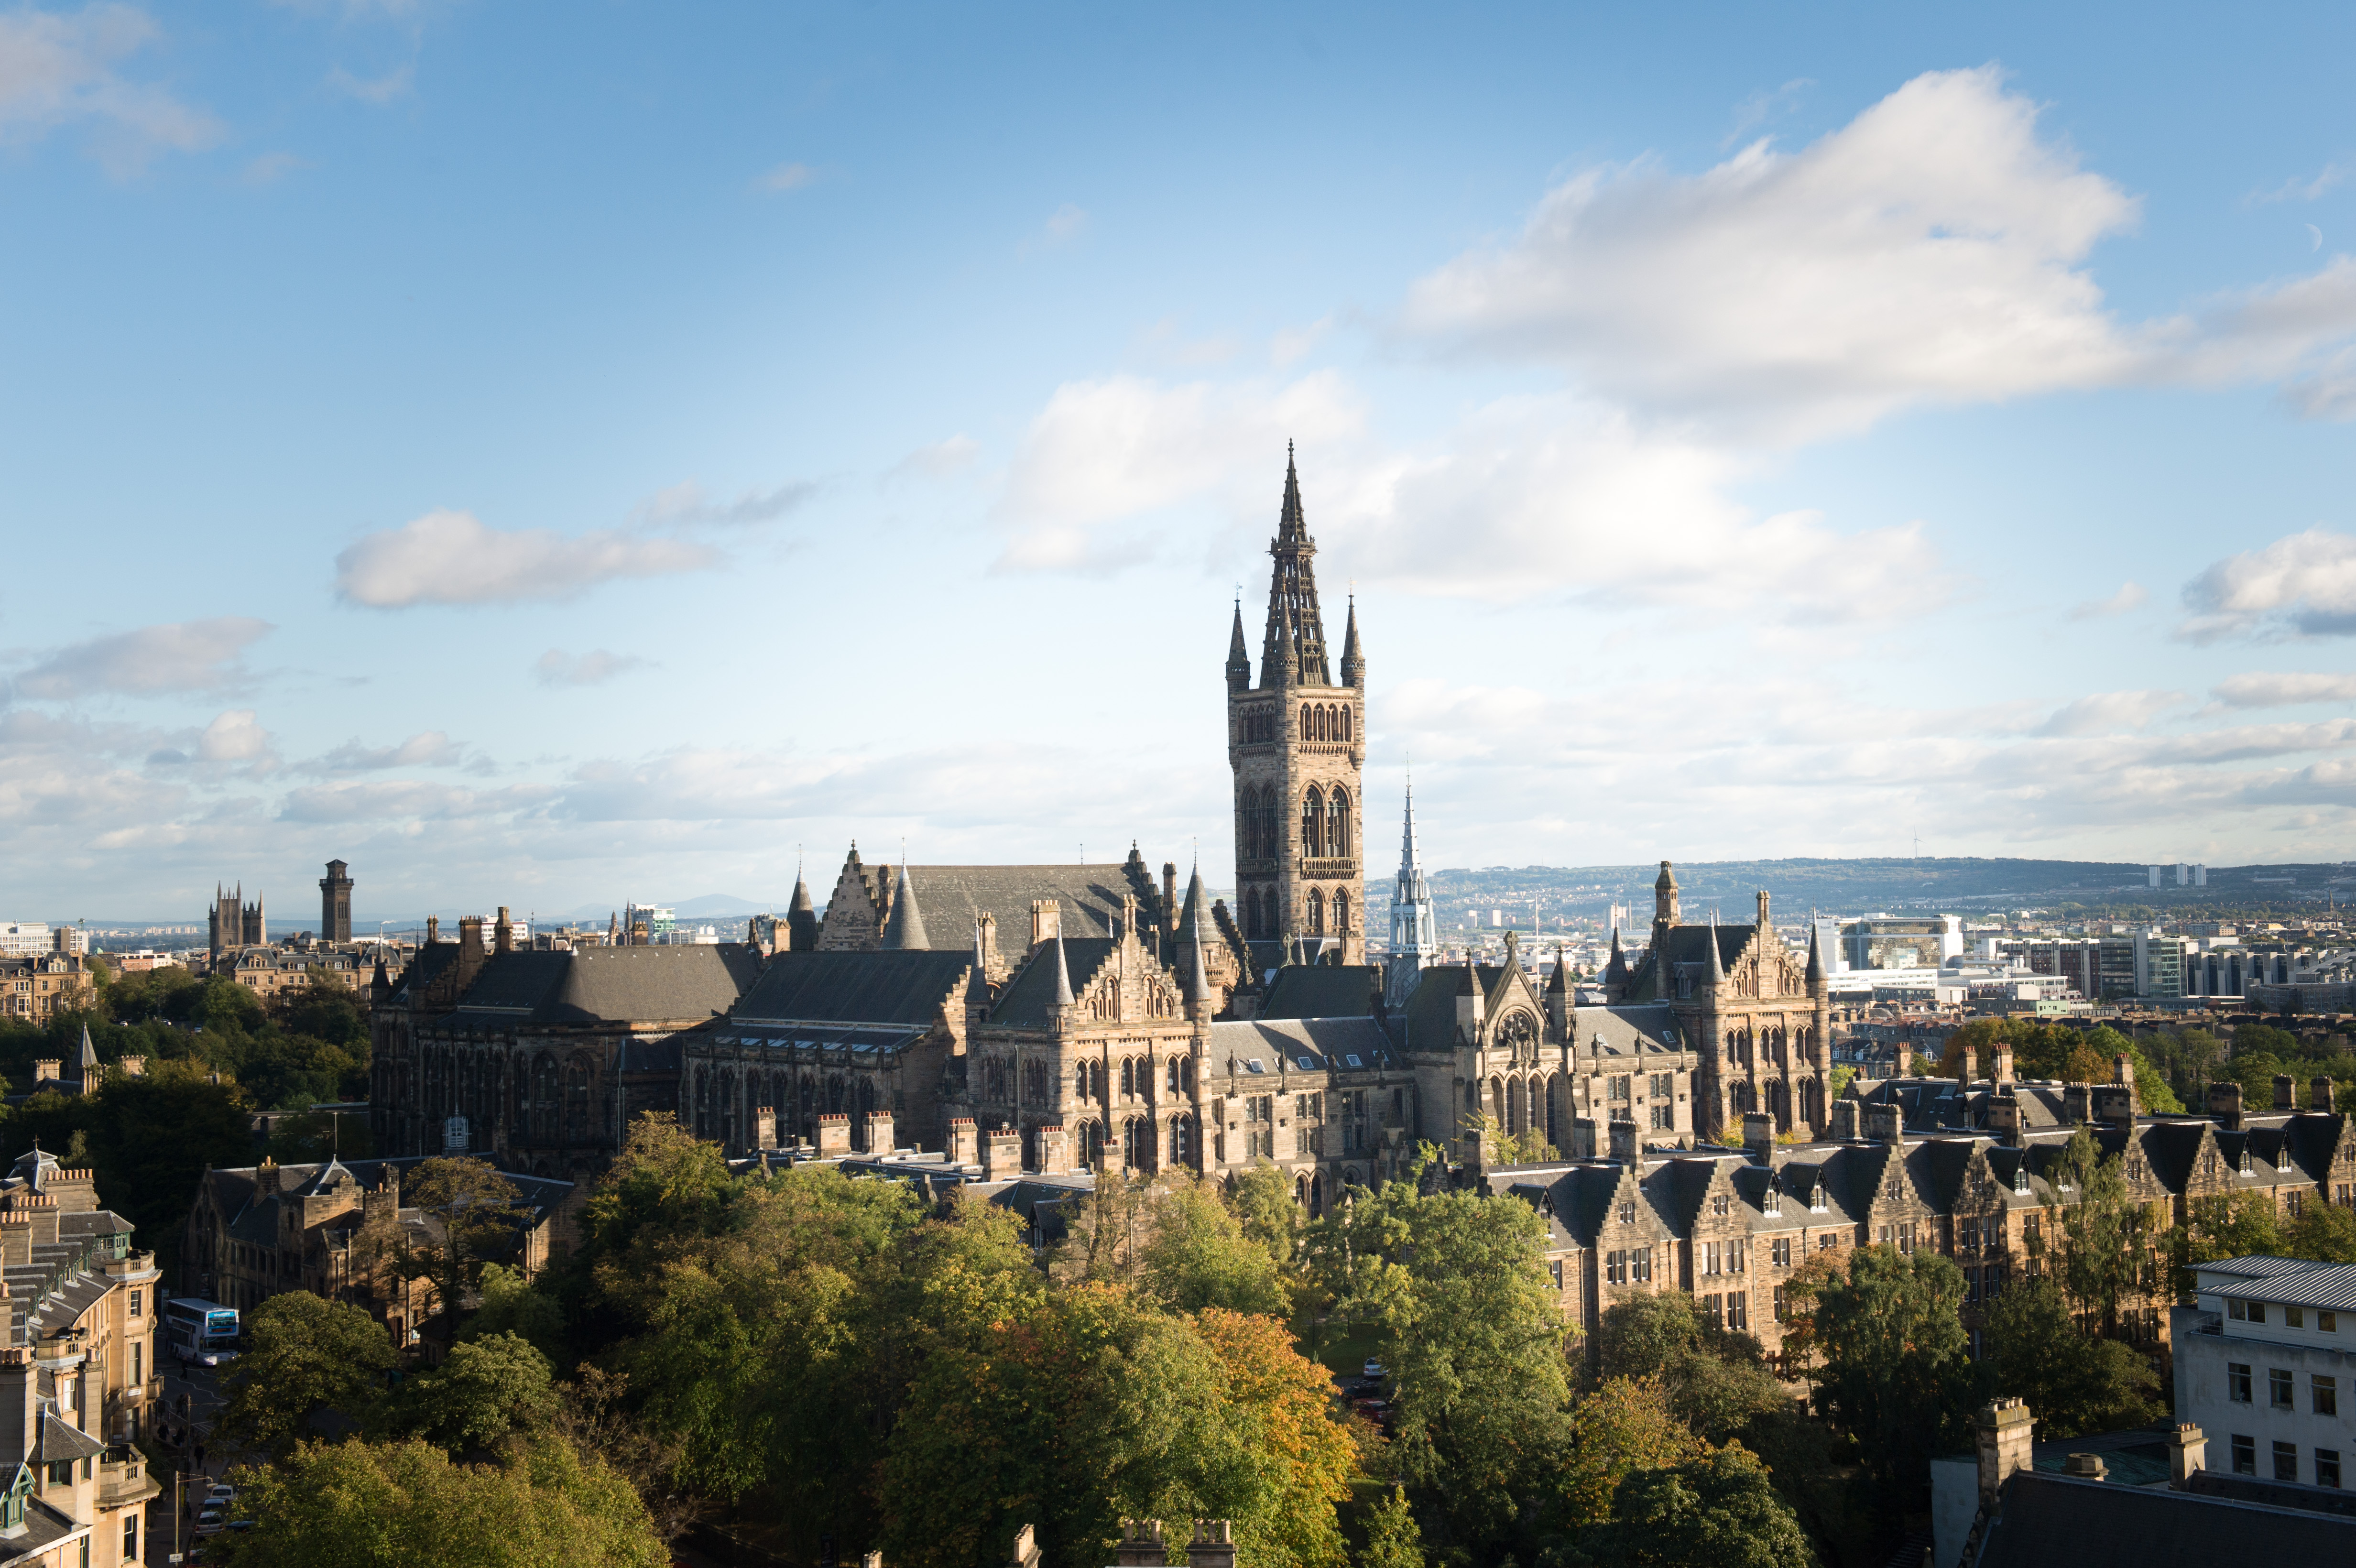
\includegraphics[keepaspectratio=true, width=\paperwidth]{background.jpg}};
    }
    \begin{frame}[plain,noframenumbering]
        \titlepage
    \end{frame}
}

\section{Subgraph Isomorphism}

\begin{frame}{Non-Induced Subgraph Isomorphism}

    \begin{center}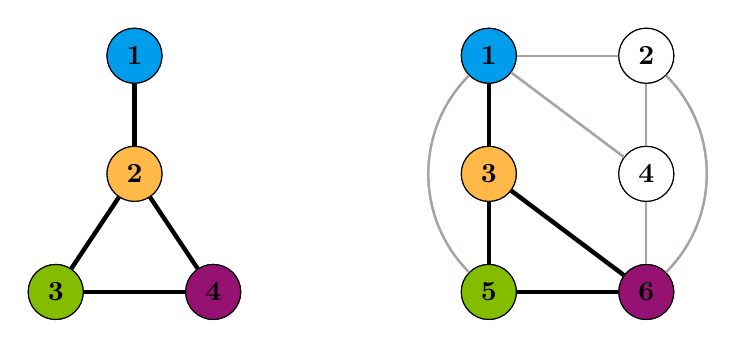
\begin{tikzpicture}
        \node <1> [draw, circle, fill=white, inner sep=4pt, font=\bfseries] (Na) at (1,  0) {1};
        \node <1> [draw, circle, fill=white, inner sep=4pt, font=\bfseries] (Nb) at (1, -1.5) {2};
        \node <1> [draw, circle, fill=white, inner sep=4pt, font=\bfseries] (Nc) at (0, -3) {3};
        \node <1> [draw, circle, fill=white, inner sep=4pt, font=\bfseries] (Nd) at (2, -3) {4};

        \node <2> [draw, circle, fill=uofgcobalt, inner sep=4pt, font=\bfseries] (Na) at (1,  0) {1};
        \node <2> [draw, circle, fill=uofgpumpkin, inner sep=4pt, font=\bfseries] (Nb) at (1, -1.5) {2};
        \node <2> [draw, circle, fill=uofglawn, inner sep=4pt, font=\bfseries] (Nc) at (0, -3) {3};
        \node <2> [draw, circle, fill=uofgthistle, inner sep=4pt, font=\bfseries] (Nd) at (2, -3) {4};

        \draw <1> [thick, color=uofgsandstone!50] (Na) -- (Nb);
        \draw <1> [thick, color=uofgsandstone!50] (Nb) -- (Nc);
        \draw <1> [thick, color=uofgsandstone!50] (Nc) -- (Nd);
        \draw <1> [thick, color=uofgsandstone!50] (Nb) -- (Nd);

        \draw <2> [ultra thick] (Na) -- (Nb);
        \draw <2> [ultra thick] (Nb) -- (Nc);
        \draw <2> [ultra thick] (Nc) -- (Nd);
        \draw <2> [ultra thick] (Nb) -- (Nd);

        \node <1> [draw, circle, fill=white, inner sep=4pt, font=\bfseries] (N1) at (5.5,  0) {1};
        \node <1> [draw, circle, fill=white, inner sep=4pt, font=\bfseries] (N2) at (7.5,  0) {2};
        \node <1> [draw, circle, fill=white, inner sep=4pt, font=\bfseries] (N3) at (5.5, -1.5) {3};
        \node <1> [draw, circle, fill=white, inner sep=4pt, font=\bfseries] (N4) at (7.5, -1.5) {4};
        \node <1> [draw, circle, fill=white, inner sep=4pt, font=\bfseries] (N5) at (5.5, -3) {5};
        \node <1> [draw, circle, fill=white, inner sep=4pt, font=\bfseries] (N6) at (7.5, -3) {6};

        \node <2> [draw, circle, fill=uofgcobalt, inner sep=4pt, font=\bfseries] (N1) at (5.5,  0) {1};
        \node <2> [draw, circle, fill=white, inner sep=4pt, font=\bfseries] (N2) at (7.5,  0) {2};
        \node <2> [draw, circle, fill=uofgpumpkin, inner sep=4pt, font=\bfseries] (N3) at (5.5, -1.5) {3};
        \node <2> [draw, circle, fill=white, inner sep=4pt, font=\bfseries] (N4) at (7.5, -1.5) {4};
        \node <2> [draw, circle, fill=uofglawn, inner sep=4pt, font=\bfseries] (N5) at (5.5, -3) {5};
        \node <2> [draw, circle, fill=uofgthistle, inner sep=4pt, font=\bfseries] (N6) at (7.5, -3) {6};

        \draw <1> [thick, color=uofgsandstone!50] (N1) -- (N2);
        \draw <1> [thick, color=uofgsandstone!50] (N1) -- (N3);
        \draw <1> [thick, color=uofgsandstone!50] (N1) -- (N4);
        \draw <1> [thick, color=uofgsandstone!50] (N2) -- (N4);
        \draw <1> [thick, color=uofgsandstone!50] (N3) -- (N5);
        \draw <1> [thick, color=uofgsandstone!50] (N3) -- (N6);
        \draw <1> [thick, color=uofgsandstone!50] (N4) -- (N6);
        \draw <1> [thick, color=uofgsandstone!50] (N5) -- (N6);
        \draw <1> [thick, color=uofgsandstone!50] (N2) to [in=45, out=315] (N6);
        \draw <1> [thick, color=uofgsandstone!50] (N1) to [in=135, out=225] (N5);

        \draw <2> [thick, color=uofgsandstone!50] (N1) -- (N2);
        \draw <2> [ultra thick] (N1) -- (N3);
        \draw <2> [thick, color=uofgsandstone!50] (N1) -- (N4);
        \draw <2> [thick, color=uofgsandstone!50] (N2) -- (N4);
        \draw <2> [ultra thick] (N3) -- (N5);
        \draw <2> [ultra thick] (N3) -- (N6);
        \draw <2> [thick, color=uofgsandstone!50] (N4) -- (N6);
        \draw <2> [ultra thick] (N5) -- (N6);
        \draw <2> [thick, color=uofgsandstone!50] (N2) to [in=45, out=315] (N6);
        \draw <2> [thick, color=uofgsandstone!50] (N1) to [in=135, out=225] (N5);
    \end{tikzpicture}\end{center}

\end{frame}

\begin{frame}{Benchmark Instances}

    \begin{itemize}
        \item Other papers: a subset of 5,725 instances from Christine Solnon's selection:
            \begin{itemize}
                \item Randomly generated with different models.
                \item Real-world graphs.
                \item Computer vision problems.
                \item Biochemistry problems.
                \item Phase transition instances.
            \end{itemize}
        \item Here: all 14,621 instances:
            \begin{itemize}
                \item $\ge \input{../paper/gen-n-sat.tex}$ satisfiable.
                \item $\ge \input{../paper/gen-n-unsat.tex}$ unsatisfiable.
            \end{itemize}
        \item A lot of them are very easy for good algorithms.
    \end{itemize}

\end{frame}

\begin{frame}{The Algorithm}

    \begin{itemize}
        \item A variable for every pattern vertex.
        \item Domains range over target vertices.
        \item Clever filtering at the top of search using neighbourhood degree sequences and paths.
        \item Bit-parallel forward checking search:
            \begin{itemize}
                \item Adjacency and pre-computed path count constraints.
                \item Cheap hacky all-different propagator.
                \item Smallest domain first, tie-breaking on highest degree.
            \end{itemize}
    \end{itemize}

\end{frame}

\begin{frame}{Is It Any Good?}

    \includegraphics<1>{gen-graph-others.pdf}%
    \includegraphics<2>{gen-graph-others-zoom.pdf}

\end{frame}

\begin{frame}{Value-Ordering Heuristics}
    \begin{itemize}
        \item Highest static degree first.
        \item But degree spread is usually quite low\ldots
    \end{itemize}
\end{frame}

\begin{frame}{Sanity Check}

    \includegraphics<1>{gen-graph-value-ordering-heuristics.pdf}%
    \includegraphics<2>{gen-graph-value-ordering-heuristics-unsat.pdf}%

\end{frame}

\begin{frame}{Discrepancy Search}

    \includegraphics<1>{gen-graph-scatter-dds.pdf}

\end{frame}

\begin{frame}{Restarts and Nogoods}

    \begin{itemize}
        \item Restarts to affect \emph{value}-ordering heuristics.
        \item Two watched literals to avoid repeating ourselves.
        \item Luby with a magic constant multiplier.
            \begin{itemize}
                \item 666, chosen by divine revelation.
            \end{itemize}
    \end{itemize}

\end{frame}

\begin{frame}{Random Value-Ordering with Restarts}

    \includegraphics<1>{gen-graph-random-restarts.pdf}%
    \includegraphics<2>{gen-graph-scatter-random.pdf}

\end{frame}

\begin{frame}{Biased Value-Ordering}

    \only<1>{
    \begin{itemize}
        \item Select a vertex $v'$ from the chosen domain $D_v$ with
            probability \[ p(v') = \frac{2^{\deg(v')}}{\sum_{w \in D_v}{2^{\deg(w)}}} \text{.} \]
        \item Looks a lot like $\mathit{softmax}$, which uses base $e$.
    \end{itemize}
    }%
    \includegraphics<2>{gen-graph-value-ordering-heuristics-biased.pdf}%
    \includegraphics<3>{gen-graph-scatter-biased.pdf}

\end{frame}

\begin{frame}{Biased Value-Ordering with Restarts}

    \includegraphics<1>{gen-graph-restarts.pdf}%
    \includegraphics<2>{gen-graph-scatter-final.pdf}

\end{frame}

\section{Maximum Common Subgraph}

\begin{frame}{Maximum Common Subgraph Algorithms}

    \includegraphics<1>{gen-graph-mcs.pdf}%
    \includegraphics<2>{gen-graph-scatter-kdown.pdf}%
    \includegraphics<3>{gen-graph-scatter-mcsplit.pdf}%

\end{frame}

\section{Parallel}

\begin{frame}{Parallel}

    \includegraphics<1>{gen-graph-parallel.pdf}%
    \includegraphics<2>{gen-graph-as-parallel.pdf}%
    \includegraphics<3>{gen-graph-scatter-parallel.pdf}%

\end{frame}

\begin{frame}{Properties of This Sort of Parallel Search}
    \begin{itemize}
        \item Reproducible (assuming each thread has its own deterministic random number generator)
        \item Can perform worse than sequential on satisfiable instances:
            \begin{itemize}
                \item Nogoods can knock out values from domains, leading to a different random
                    search order, even if the first thread uses the same seed.
                \item Challenge for you: design a sane and fast biased random selection algorithm
                    that is immune to this, and that is statistically the same sequentially. It
                    feels like this should be possible\ldots
                \item Also, our all different propagator isn't monotonic or idempotent.
            \end{itemize}

        \item Similarly, adding extra threads can make it worse.
    \end{itemize}
\end{frame}

\begin{frame}[plain,noframenumbering]
    \begin{center}
        \vspace*{4em}
        \url{http://www.dcs.gla.ac.uk/~ciaran} \\
        \vspace{1em}
        \href{mailto:ciaran.mccreesh@glasgow.ac.uk}{\nolinkurl{ciaran.mccreesh@glasgow.ac.uk}} \\
    \end{center}

    \begin{tikzpicture}[remember picture, overlay]
        \node at (current page.north west) {
            \begin{tikzpicture}[remember picture, overlay]
                \fill [fill=uofguniversityblue, anchor=north west] (0, 0) rectangle (\paperwidth, -2.6cm);
            \end{tikzpicture}
        };

        \node (logo) [anchor=north east, shift={(-0.6cm,-0.6cm)}] at (current page.north east) {
            
\includegraphics[keepaspectratio=true,scale=0.7]{UoG_keyline.pdf}
        };
    \end{tikzpicture}
\end{frame}

\end{document}

